\section{Benchmark design}

\subsection{Systems under test}

\sys evaluates retrieval infrastructure for agentic memory decisions. The paper matrix runs all experiments on one CPU-only operator workstation so quality, latency, throughput, and context-cost proxy values are measured under the same hardware/runtime profile. The reportable engine set contains FAISS CPU \citep{johnson2019faiss}, LanceDB in-process \citep{lancedb}, PostgreSQL with pgvector \citep{pgvector}, and Qdrant \citep{qdrant}. LanceDB service mode is listed but excluded from the paper matrix because the conformance table has no passing local service row.

\sys is organized as a decision-audit pipeline: a reported winner is tied to a stated conformance gate, workload, objective, and run budget. The engine set covers four representative local operating modes: an exact in-process baseline, an embedded/local store, a PostgreSQL extension, and a service vector database. FAISS CPU serves as an exact in-process local baseline and deployment option. The adapter contract is the extension path for additional engines such as Milvus, Weaviate, Redis, Vespa, OpenSearch, or Chroma.

Every reportable engine must pass the same adapter contract before its runs can enter paper-facing tables. The contract covers lifecycle operations, bulk and incremental writes, query and batch query, vector and payload updates, delete semantics, flush or commit behavior, index controls, and minimum stats fields. The conformance suite checks CRUD correctness, post-flush visibility, filter correctness, update semantics, delete semantics, and streaming-memory post-insert retrievability semantics. This gate prevents a benchmark table from silently mixing engines with different unsupported behavior and reports missing conformance as an explicit exclusion.

\begin{figure}[t]
  \centering
  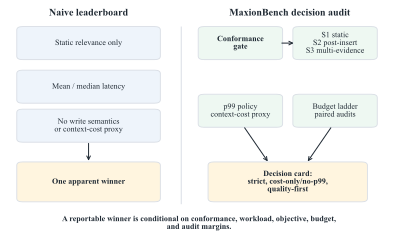
\includegraphics[width=\linewidth]{../figures/maxionbench_decision_audit_conceptual.svg}
  \caption{From leaderboard evaluation to decision audit. \sys makes a deployment choice reportable only after conformance, workload evidence, p99 policy, context-cost accounting, budget stability, and paired margins are all visible.}
  \label{fig:protocol-schematic}
\end{figure}

\subsection{Workloads}

\sys uses three workloads designed to isolate retrieval-infrastructure behavior that matters to agentic applications. S1 (single-hop static retrieval) evaluates SciFact and FiQA through local BEIR-format bundles \citep{thakur2021beir,wadden2020scifact,maia2018fiqa}; its primary quality metric is \ndcg. S2 (streaming retrieval with post-insert probes) combines a deterministic 50K-passage static background from the same source family with a CRAG-500 event stream \citep{facebookcrag}; it reports static \ndcg{} and post-insert top-10 retrievability probes at one and five seconds after insert acknowledgment. S3 (multi-evidence HotpotQA retrieval) uses \hotpotmaxionbench{}, a frozen preprocessing of the HotpotQA dev distractor split, and measures whether the retrieved top-10 contains the supporting evidence set with \ecov. \hotpotmaxionbench{} contains 7{,}405 questions; the paper-facing S3 multi-evidence matched audit uses the configured 5{,}000-query subset recorded by the run configuration.

\begin{table}[t]
\centering
\scriptsize
\setlength{\tabcolsep}{2pt}
\caption{MaxionBench workload summary. S1 single-hop and S2 streaming counts come from the processed local BEIR-format bundles under the 50K-document paper cap; S3 multi-evidence counts come from the HotpotQA-MaxionBench manifest. Cov@10 denotes \ecov{}, and all-hit@10 denotes all\_evidence\_hit@10.}
\label{tab:workload-summary}
\begin{tabularx}{\linewidth}{@{}>{\raggedright\arraybackslash}p{0.08\linewidth}>{\raggedright\arraybackslash}p{0.13\linewidth}>{\raggedright\arraybackslash}p{0.12\linewidth}>{\raggedright\arraybackslash}p{0.13\linewidth}>{\raggedright\arraybackslash}p{0.09\linewidth}>{\raggedright\arraybackslash}p{0.22\linewidth}>{\raggedright\arraybackslash}p{0.15\linewidth}@{}}
\toprule
Workload & Assets & Corpus & Queries / events & Labels & Decision role & Metrics \\
\midrule
S1 & BEIR-format SciFact + FiQA & 50{,}000 docs & 894 queries & 1{,}685 qrels & static relevance and tail-latency baseline & \ndcg{} \\
S2 & 50K BEIR background + CRAG-500 stream & 50{,}000 background + 500 inserted stream passages & 894 static queries; 500 stream events & 1{,}685 static qrels; 500 event qrels & post-insert retrievability diagnostic under a write stream & \ndcg{}; post-insert@1s/5s \\
S3 & \hotpotmaxionbench{} from HotpotQA dev distractor & 66{,}635 docs & 7{,}405 questions; 5{,}000-query matched-audit subset & 14{,}810 qrels & multi-evidence and context-cost decision stress & Cov@10; all-hit@10 \\
\bottomrule
\end{tabularx}
\end{table}

The experiments use fixed read/write-client settings so latency, throughput, and post-insert probes are comparable across engines. S1 single-hop and S3 multi-evidence evaluate read-client settings $\{1,4,8\}$. S2 streaming uses eight read clients and two serialized write clients, then probes each inserted event passage at $T+1s$ and $T+5s$, where $T$ is the time at which the adapter's insert plus flush path returns. Each workload is evaluated with two local embedding tiers, \texttt{BAAI/bge-small-en-v1.5} and \texttt{BAAI/bge-base-en-v1.5} \citep{bge}. We write bge-small and bge-base after first mention.

\subsection{Metrics and decisions}

\sys reports quality, tail latency, throughput, a normalized context-cost proxy, and stability across budget levels. Latency is measured on precomputed query vectors and times \texttt{adapter.query} plus top-k materialization, including service/container overhead inside the adapter call when applicable; offline embedding is excluded from latency and included only in the context-cost proxy. We rank latency by \maxrowp: the maximum observed p99 across the configured B2 read-client or read/write-client rows and repeats for a candidate. We report this audit statistic with the recorded hardware/runtime profile. For S1 single-hop and S2 streaming, quality is \ndcg. For S3 multi-evidence, quality is
\[
\mathrm{evidence\_coverage@k}(q)=\frac{|E(q)\cap R_k(q)|}{|E(q)|},
\]
where $E(q)$ is the gold evidence set and $R_k(q)$ is the retrieved top-$k$ set. For S2 streaming, \(\mathrm{post\_insert\_hit@10,\Delta}\) is one when the newly inserted supporting passage appears in $R_{10}(q,T+\Delta)$ for $\Delta\in\{1s,5s\}$ after the adapter's insert-plus-flush path returns. This agent-facing metric evaluates retrievability after acknowledgement; low-level index visibility is outside the metric. For S2 streaming, the strict-latency rule gates on static nDCG@10 and reports \texttt{post\_insert\_hit@10,1s} and \texttt{post\_insert\_hit@10,5s} as agent-facing write/retrieve diagnostics. We therefore interpret S2 streaming deployment choices as static-quality/cost/p99 decisions accompanied by post-insert retrievability evidence.

Within each workload and configured subset, all reportable engines evaluate the same quality query or event IDs; latency and throughput observation counts may differ because they are measured in timed windows. Paired audits join explicitly by query ID or event index. Quality differences across engines therefore reflect configured search behavior, tie handling, filtering/update semantics, and top-k materialization under the adapter contract rather than differences in the embedding model itself. In the reported MaxionBench matrix, the FAISS CPU rows have empty \texttt{index\_params} and therefore use the adapter's exact flat index; recorded \texttt{hnsw\_ef} sweep values are not consumed by that flat-index path.

The deployment rule is deliberately simple. A strict-latency survivor must pass the conformance gate, satisfy the workload quality floor recorded in the run configuration, and remain below the stated \maxrowp cap. For each workload, engine, and embedding tier, these survivors are ranked by the normalized context-cost proxy
\[
\mathrm{task\_cost\_est}=C_{\mathrm{retrieval}}+C_{\mathrm{embedding}}+c_{\mathrm{llm\_in}}\cdot N_{\mathrm{retrieved\_input\_tokens}},
\]
with lower \maxrowp and higher throughput used as tie-breaks. The report field is named \texttt{task\_cost\_est}, but the paper interprets it only as a normalized context-token cost proxy: it is not a cloud-dollar estimate. In the reported local run, \(C_{\mathrm{embedding}}=0\) for offline embeddings and \(c_{\mathrm{llm\_in}}=0.15\) is a project-defined token coefficient. The strict-latency objective selects the lowest-cost survivor under the 200 ms \maxrowp cap used as the main audit policy. The report also exposes cost-only/no-p99 and quality-first objectives because those plausible operator choices can select different configurations.

\begin{center}
\fbox{\begin{minipage}{0.92\linewidth}
\footnotesize
\textbf{Decision-card protocol.} Given engines \(E\), embedding tiers \(M\), workloads \(W\), budget levels \(B\), a p99 cap \(\tau\), and objectives \(O\), \sys runs the following audit:
\begin{enumerate}[leftmargin=*,nosep]
  \item run adapter conformance checks for each engine and exclude non-conforming rows;
  \item evaluate quality, \maxrowp, throughput, and context-cost proxy for each workload and embedding tier;
  \item rank surviving configurations under each stated objective and record strict-latency, cost-only/no-p99, and quality-first choices;
  \item compute B0/B1/B2 stability statistics and run paired audits for high-risk aggregate margins;
  \item emit a decision card with choices, margins, stability, conformance status, and interpretation notes.
\end{enumerate}
\end{minipage}}
\end{center}

\subsection{Budget ladder}

The benchmark uses three budget levels to test whether decisions are stable under shorter budgeted runs. B0 uses 10 seconds of warmup, 10 seconds of measurement, and one repeat. B1 uses 15 seconds of warmup, 30 seconds of measurement, and one repeat. B2 uses 30 seconds of warmup, 60 seconds of measurement, and two repeats. Stability is reported as Spearman rank correlation, top-1 agreement, and top-2 agreement between budget-level rankings. This design turns budget instability into a reported experimental outcome.
